\chapter{What is Blazon?}

Blazon is the language of heraldry and family crests, it dates back to the twelfth century and provides a strict set of rules about how to produce a coat of arms.  
There are several different versions of Blazon found around Europe however all follow the same behavioural rules regarding tinctures and charges.  Most versions differ only in the set of tinctures and honourable ordinaries either having a more generous or conservative view on what is and isn't acceptable for example, African Blazon allows for an Orange coloured Tincture whilst English Blazon does not.
For this project I focused on exclusively on a strict English Blazon.  


Blazon is a powerful language for allowing limitless combinations and configurations of patterns and shapes to be \emph{Blazoned} onto a shield in and recorded in a concise textual description.

What is impressive about the language is that it achieves this flexibility whilst reaming fairly formal and well defined, 
restricting the set of tinctures to total seven and maintaining a fairly low number of pre-defined honourable ordinaries. 

Blazon, like any other language, has some unique terminology used to address certain aspects of heraldry.  Anyone attempting utilize the language will need to familiarise themselves with this terminology.    

\section{The Seven Tinctures}
The most fundamental elements of Blazon are the Tinctures.  Tinctures are the set of colours allowed in coats of arms.  English Blazon defines a set of seven tinctures and places them into to groups metals and non-metals. 

\begin{table}[The Seven Tinctures]
\centering
\begin{tabular}{| c | c | c |}

	\hline
	\multicolumn{3}{| c |}{The Seven Tinctures} \\ \hline

	Tincture & Colour & Metal \\ \hline

	Azure & Blue & Non-metal \\
	Argent & Silver & Metal \\
	Gules & Red & Non-metal \\
	Or & Gold & Metal \\
	Purpure & Purple & Non-metal \\ 
	Sable & Black & Non-metal \\
	Vert & Green & Non-metal \\
	\hline
\end{tabular}
\caption{Table of Tinctures found in English Blazon, the corresponding colours and whether each tincture is or isn't a metal.}
\label{tab:label}
\end{table}


Although at first this may seem overly restrictive Blazon overcomes having a limited set of valid tinctures by leaving interpretation of the tone and shade of each Tincture's corresponding colour to the artist producing the shield. 
An Azure, blue, shield could be a light sky blue or a dark navy shade of blue depending upon the artists preference, as long as it is recognisably blue. 

The Freedom of Interpretation is a great strength of Blazon vastly increases the different graphical variations of Blazoned shields without radically increasing the size of the language by exhaustively listing a set of valid tones and shades. 

With regard to the two metallic Tinctures Or, gold, and Argent, silver, having freedom of interpretation allows for matt, non-metallic, colours to be placed onto a shield, although they will still behave as metal Tinctures.  It is not uncommon to see yellow instead of gold and white instead of silver on many coats of arms.


\section{Furs}

Blazon incorporates several furs commonly used in coats of arms into the language.  These behave in much the same way as tinctures but don't have the same metal or non-metal property.

There are several pre-defined patterns for furs that are used directly instead of actual fur on a shield.  These patters generally consist of a repeating pattern on-top of a background colour.  Each fur has a unique pattern although several are very similar, some simply being the inverse of another.

The colours of Furs are pre-defined but can be explicitly stated as differing from the normal colours  by stating the Tinctures to be used instead.  For example for example Ermine coloured silver and black would be defined as \emph{"Ermine Argent and Sable"} 

% figure here showing furs please

\section{Fields}
A Field is simply an area on a shield.  Initially a shield has one implicit Field, which is the entire area of that shield.  Blazon allows for two operations on fields, a field can be Tinctured, with a Tincture or a Fur, or a field can be Partitioned. 
Tincturing a Field dictates that the whole area incorporated in that Field be filled in the colour of that Tincture.  Partitioning I will cover in much more detail later on.


\section{How to Blazon a Coat of Arms: Part One}

I have now defined a large enough subset of Blazon for a couple of basic examples.  

In each example we are implicitly provided with a single Field which encompasses the entire body of the shield. Then we Tincture that Field by providing a Tincture and we have successfully Blazoned a shield.  

\begin{figure}[H]
\subfigure[\emph{"Vert"}]{
\includegraphics[width=0.4\textwidth]{blazon/images/vert.eps}}
\hfill
\subfigure[\emph{"Or"}]{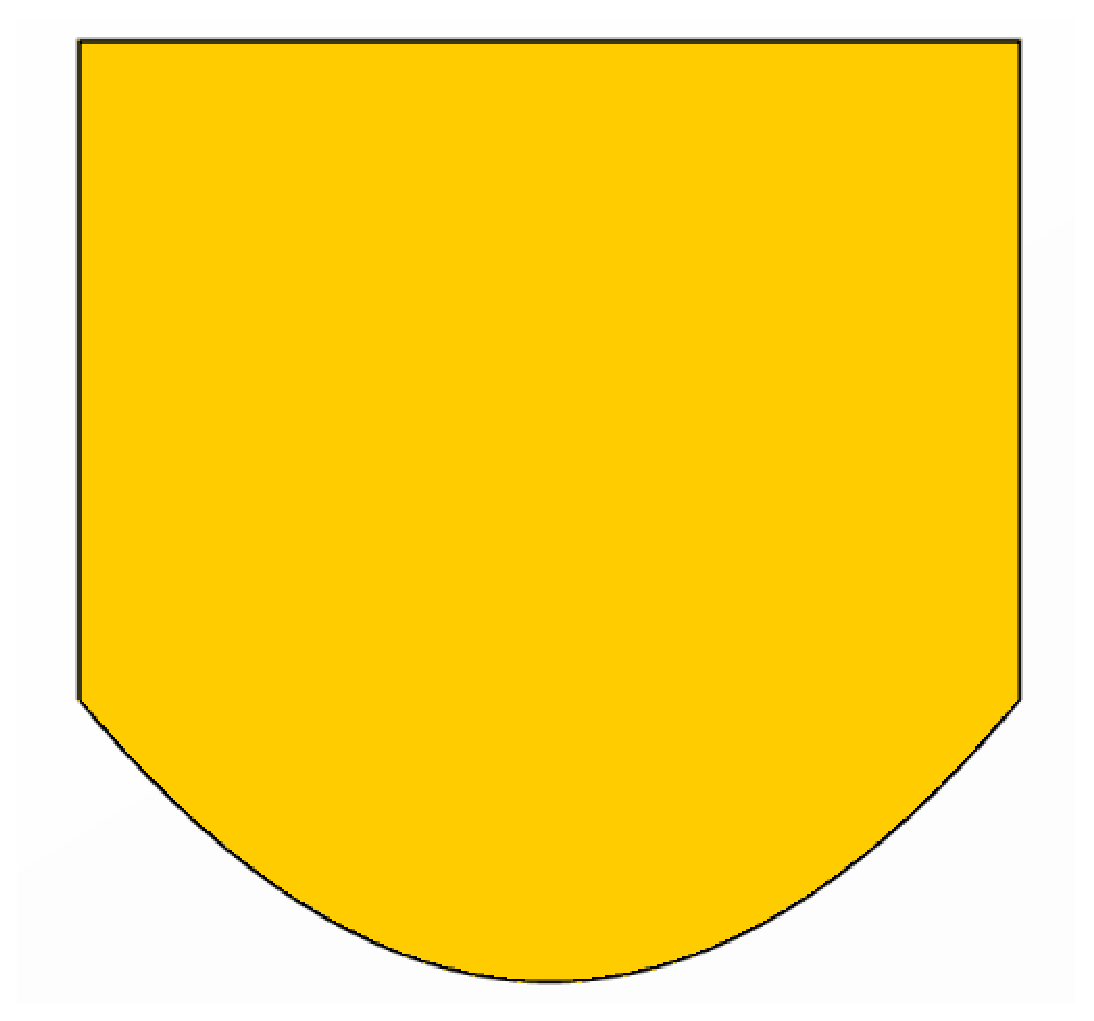
\includegraphics[width=0.4\textwidth]{blazon/images/or.eps}}
\hfill
\subfigure[\emph{"Azure"}]{
\includegraphics[width=0.4\textwidth]{blazon/images/azure.eps}}
\hfill
\subfigure[\emph{"Gules"}]{
\includegraphics[width=0.4\textwidth]{blazon/images/gules.eps}}
\hfill
\caption{Basic Blazon examples.}
\end{figure}

Although the examples in Figure 2.1 are very basic each is a complete valid Blazoning of a shield.

\section{Partitioning a Field}
The Blazon I have defined so far is very limited, only allowing for single Tincture shields.  The next natural area of the language to define is the operation of Partitioning a Field.  

As stated previously a Field can be either Tinctured or Partitioned.  To Partition a Field the key-word \emph{"Per"} is used. It is obligatory that the word immediately after \emph{"Per"} is a type of partition.  Blazon has several pre-defined partitions ranging from the very simple \emph{"Fess"} which divides a Field horizontally in half. 

Partitioning a Field divides it up into several smaller fields the number and shape of which depend on the type of Partition used.  After the Partition has been stated the Blazon sentence must go on to address the resulting new Fields. 

A shield is Implicitly Blazoned from top left to bottom right with the top most Field taking priority firstly and if two or more Fields are adjacent at the same height the left most takes priority.  

The Blazon sentence is only complete when all the Fields have been Tinctured.  If a Blazon sentence Partitions a shield into two Fields and then provides only one Tincture that sentence is Invalid.  

% figures of all the partitions 



\begin{figure}[H]
\subfigure[\emph{"Fess"}]{
\includegraphics[width=0.5\textwidth]{blazon/images/fess.eps}}
\hfill
\subfigure[\emph{"Pale"}]{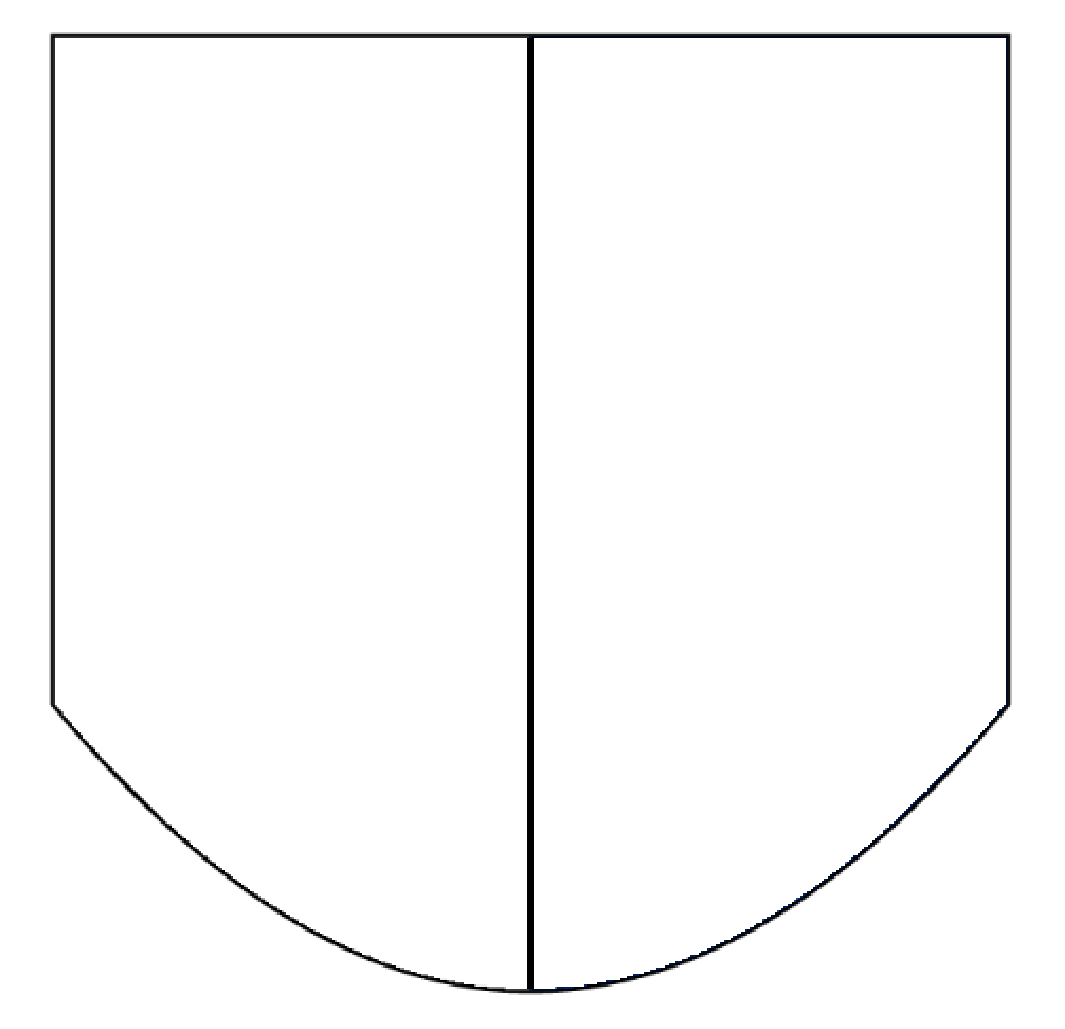
\includegraphics[width=0.5\textwidth]{blazon/images/pale.eps}}
\hfill
\subfigure[\emph{"Bend"}]{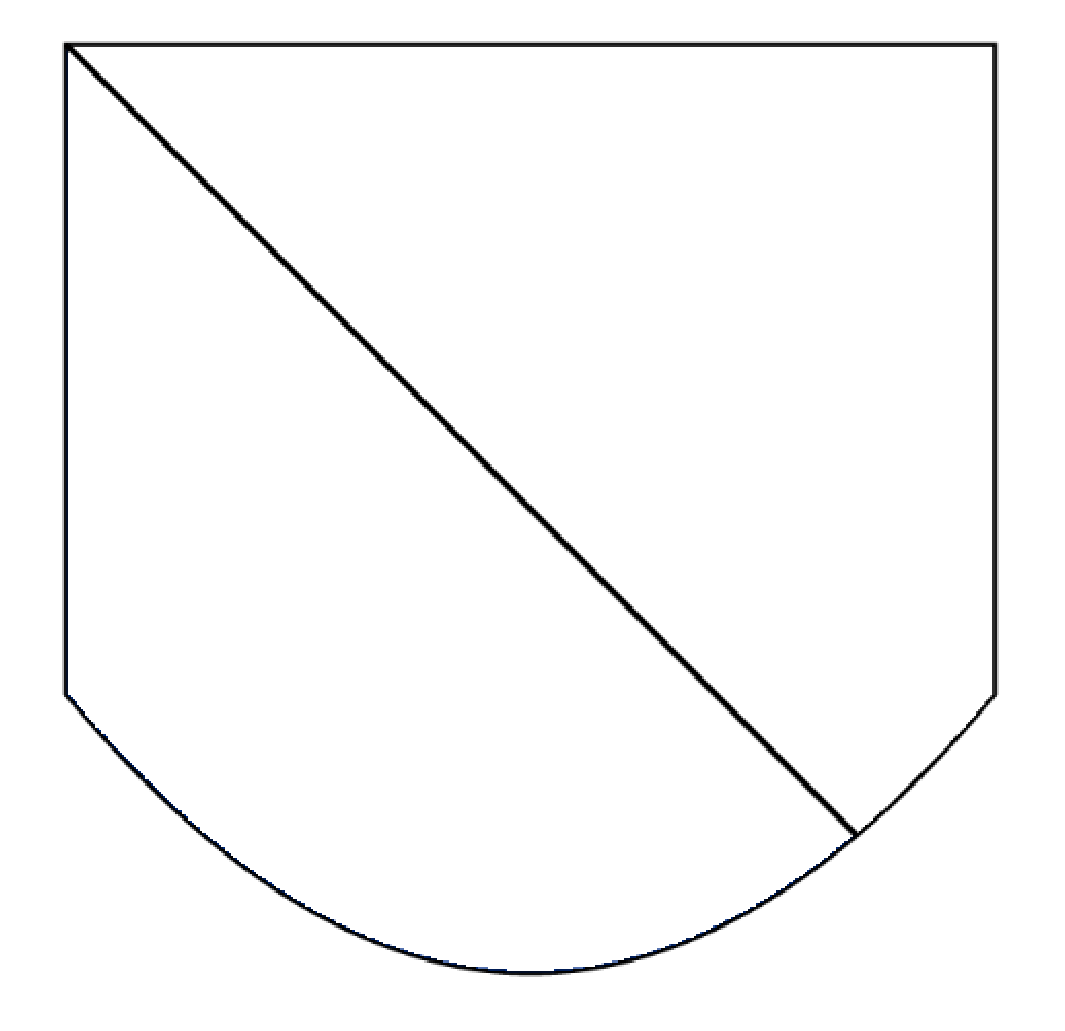
\includegraphics[width=0.5\textwidth]{blazon/images/bend2.eps}}
\hfill
\subfigure[\emph{"Bend Sinister"}]{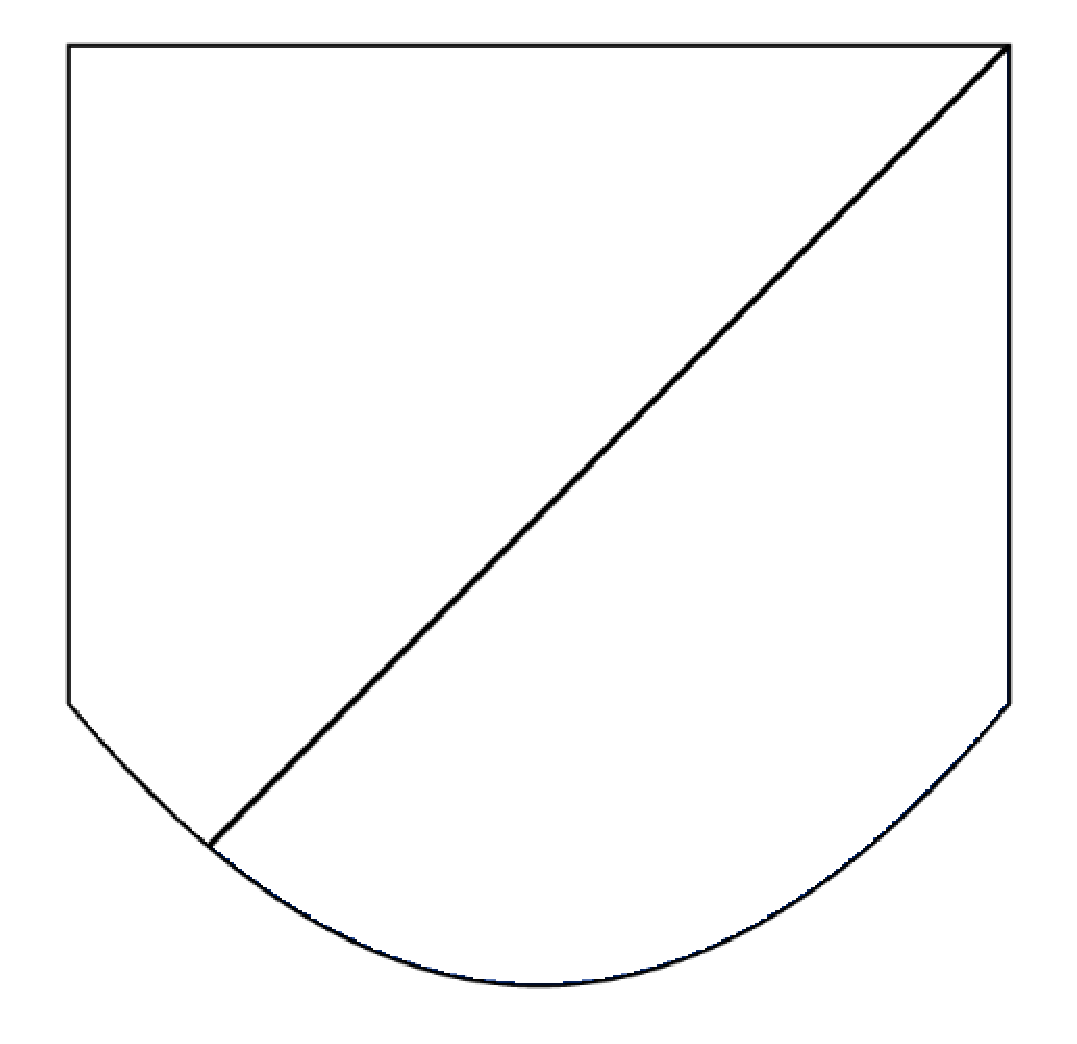
\includegraphics[width=0.5\textwidth]{blazon/images/bendsinister.eps}}
\hfill
\subfigure[\emph{"Cheveron"}]{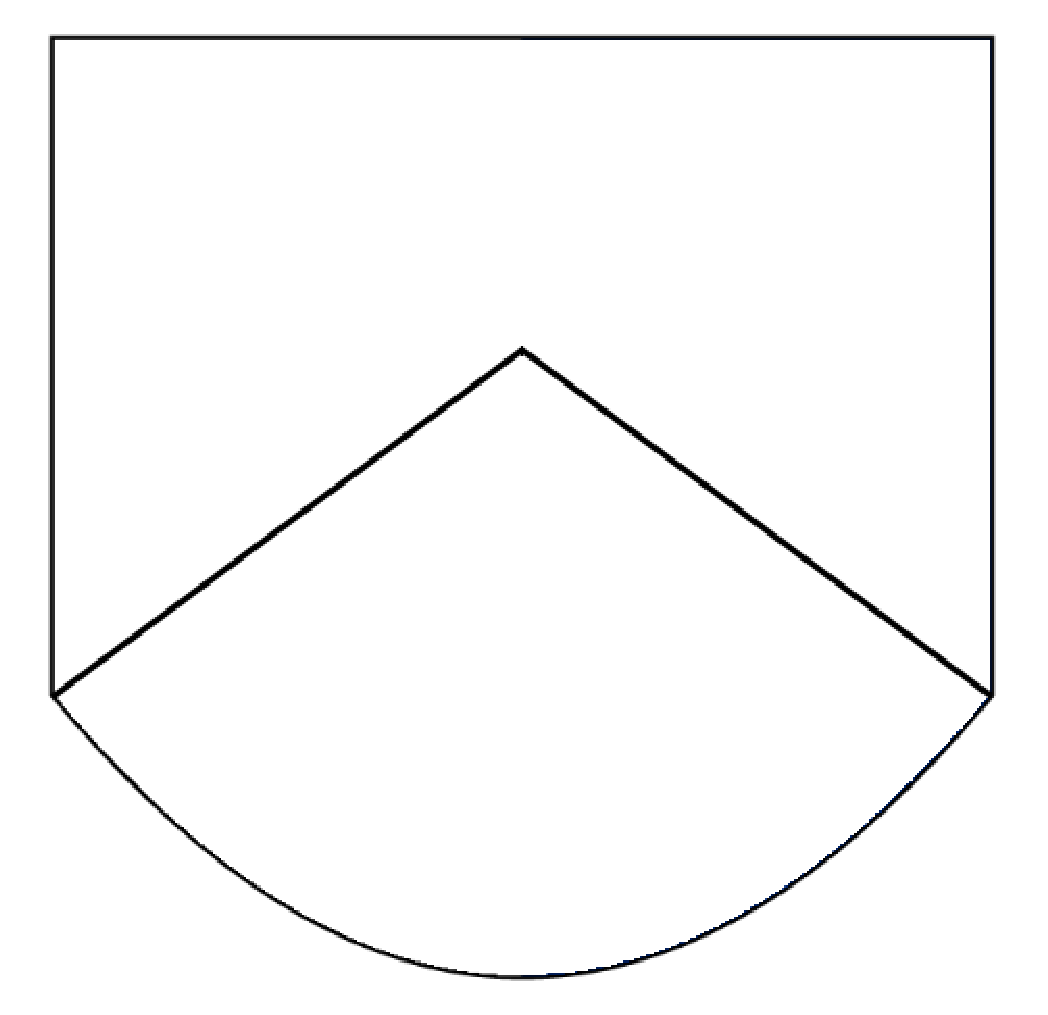
\includegraphics[width=0.5\textwidth]{blazon/images/cheveron.eps}}
\hfill
\subfigure[\emph{"Pall"}]{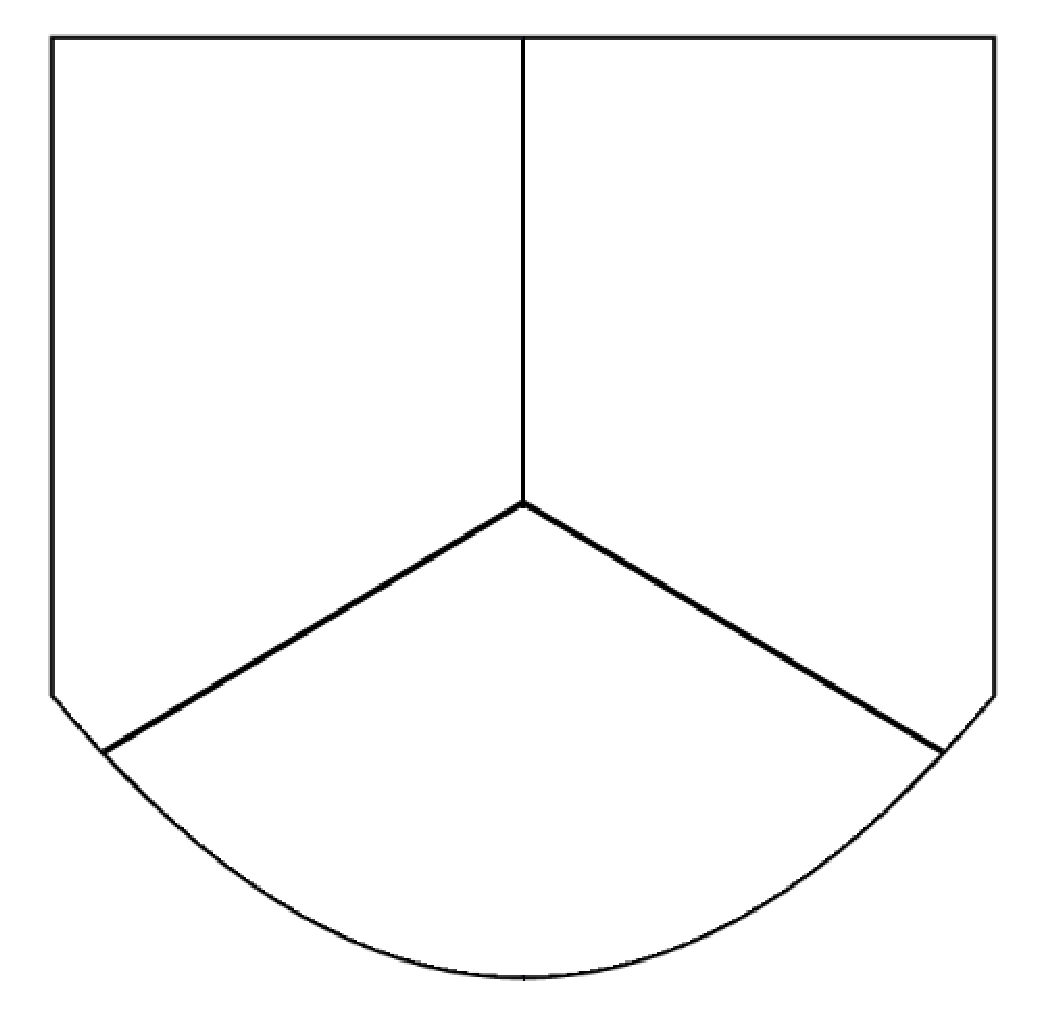
\includegraphics[width=0.5\textwidth]{blazon/images/pall.eps}}
\hfill

\caption{\emph{"Valid Partitions of a Field"}}
\end{figure}



\section{How to Blazon a Coat of Arms: Part Two}
Partitioning is a very powerful aspect of Blazon and increases the number of possible shield designs immensely.  A lot of very striking designs can be Blazoned onto a shield with very short Blazon sentences making use of Partitioning.  

The Blazon sentence,\emph{"Per Bend Gules and Azure"} Implicitly starts with a single Field which encompasses the entire body of the shield before partitioning that Field into two smaller Fields with the keyword \emph{"Per"} declaring a partition followed by the word \emph{"Bend"} which is a diagonal division of a field from top left to bottom right.  The Blazon goes onto Tincture the two new fields with the two Tinctures \emph{"Gules"} and \emph{"Azure"} respectively,  following Blazon's rule about evaluating the topmost and then leftmost field first the upper section of the shield is Tinctured \emph{"Gules"} and then the lower half is Tinctured \emph{"Azure"}.  There is no more Blazon reaming in the sentence and there are also no empty fields upon the shield, therefore this is a valid Blazon sentence and a striking red and blue shield has been produced. 


\begin{figure}[H]
\subfigure[\emph{"A single empty Field."}]{
\includegraphics[width=0.4\textwidth]{blazon/images/emptyfield.eps}}
\hfill
\subfigure[\emph{"The Field has been partitioned Per Bend"}]{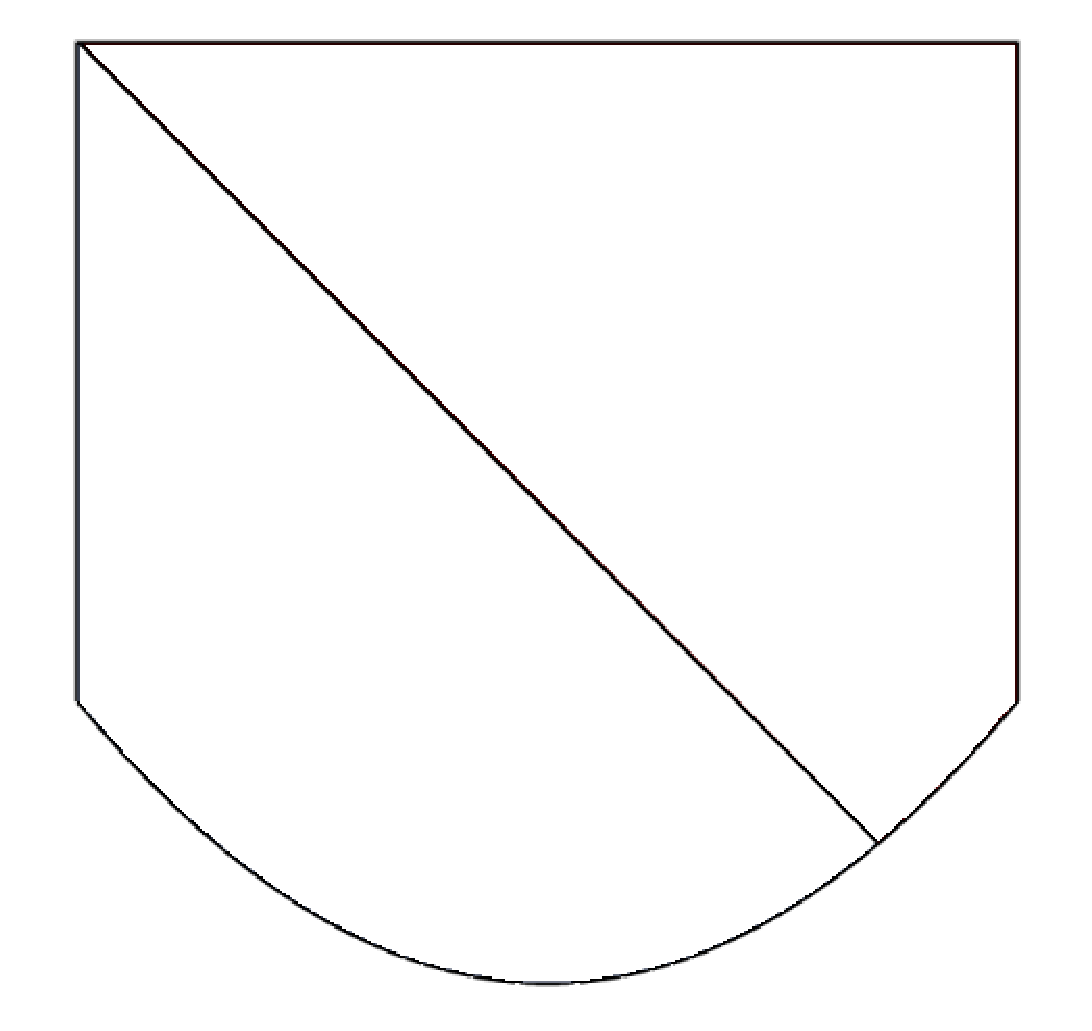
\includegraphics[width=0.4\textwidth]{blazon/images/bend.eps}}
\hfill
\subfigure[\emph{"The Topmost Field is Tinctured Gules"}]{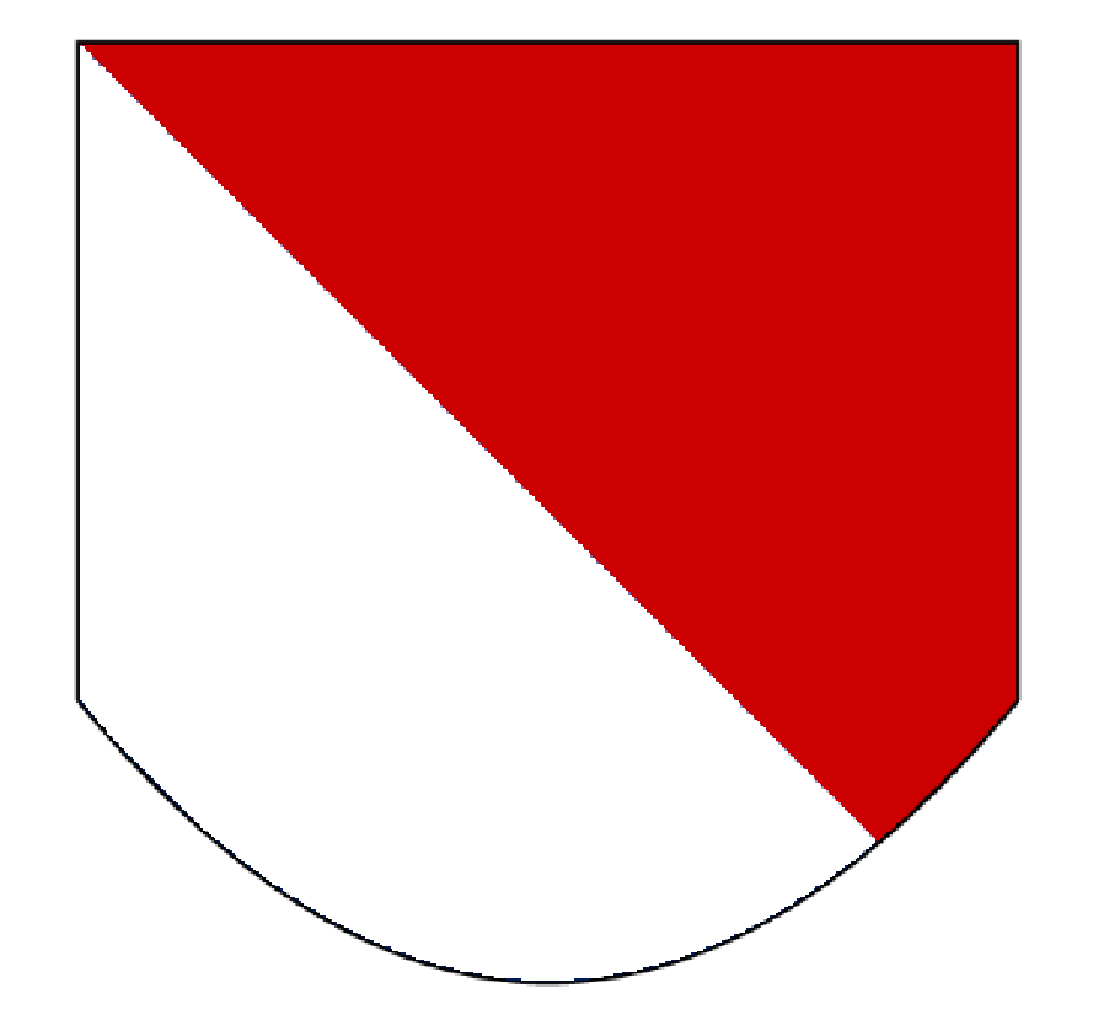
\includegraphics[width=0.4\textwidth]{blazon/images/halfdoneperbendgulesandazure.eps}}
\hfill
\subfigure[\emph{"The final Field is Tinctured Azure"}]{
\includegraphics[width=0.4\textwidth]{blazon/images/perbendgulesandazure.eps}}
\hfill
\caption{\emph{"Per Bend Gules and Azure"}.}
\end{figure}


Applying the same method as show above it is possible to validate the following Blazon sentences of similar complexity. 

\begin{figure}[H]
\subfigure[\emph{"Per Bend Sinister Argent and Vert."}]{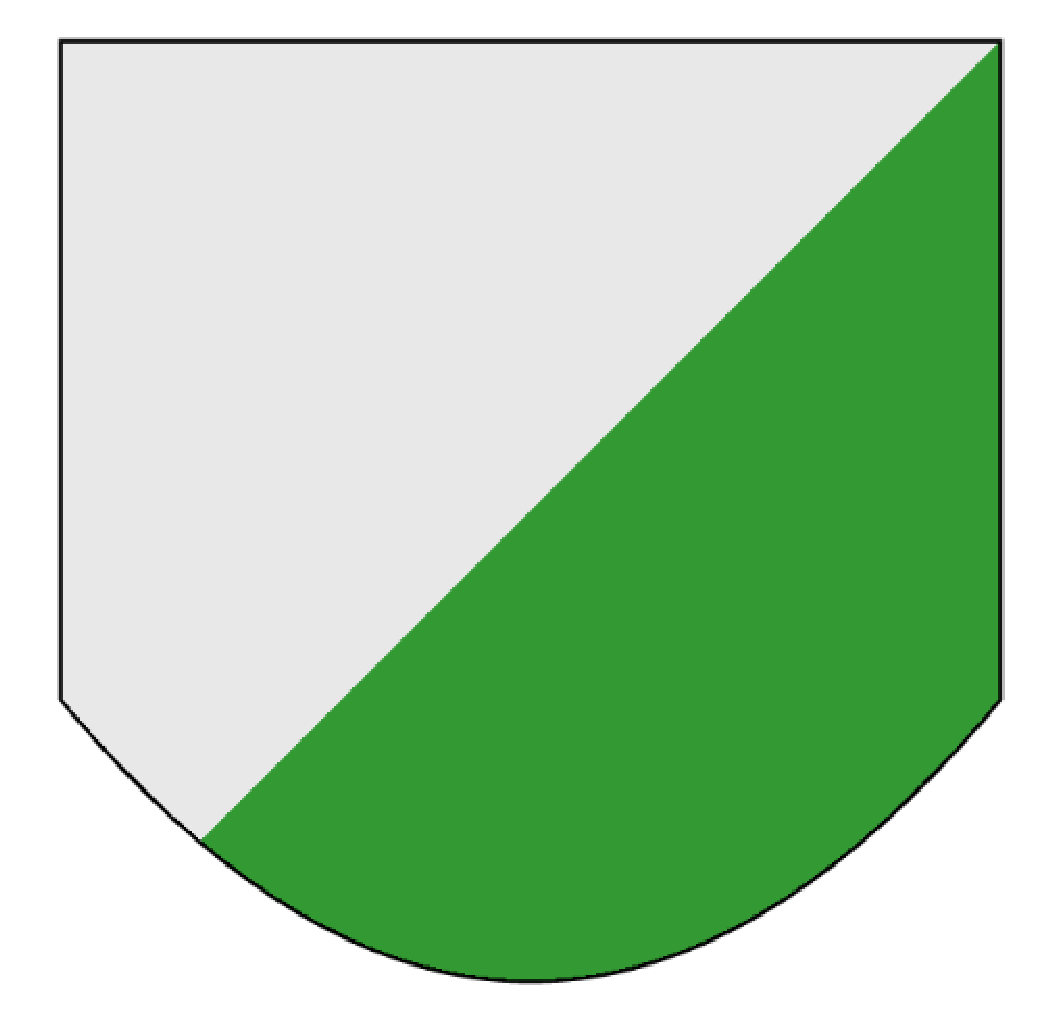
\includegraphics[width=0.4\textwidth]{blazon/images/bendsinisterargentandvert.eps}}
\hfill
\subfigure[\emph{"Per Pale Azure and Or"}]{
\includegraphics[width=0.4\textwidth]{blazon/images/perfessazureandor.examples}}
\hfill

\caption{\emph{"Two more examples of valid Blazon sentences"}.}
\end{figure}



\section{Sub-Partitioning}

Considerably more advanced patterns can be achieved buy using Sub-Partitioning.

\section{Line Types}

\section{Directions and Sides}

\section{Charges}

\section{The Rule of Tincture}
